\documentclass[10pt,a4paper]{article}
\usepackage[utf8]{inputenc}
\usepackage{amsmath}
\usepackage{amsfonts}
\usepackage{amssymb}
\usepackage{graphicx}
\author{Brock Ellefson}
\title{CSCI338 HW3}
\begin{document}
\maketitle

\section{Context-Free Grammers}
\subsection{$\lbrace$ a$^{n}$b$^{m}$ $\mid$ n $\neq$ 2m $\rbrace$}
	S $\rightarrow$ aaSb $\mid$ A $\mid$ B \\
	A $\rightarrow$ aA $\mid$ a \\
	B $\rightarrow$ bB $\mid$ b
	
\subsection{$\lbrace$ a$^{i}$ b$^{j}$ c$^{k}$ $\mid$ i, j, k $\geq$ 0 j = k or j = i $\rbrace$}
	S $\rightarrow$ $S_{1}$ $\mid$ $S_{2}$ \\
	$S_{1}$  $\rightarrow$ ab$S_{1}$ $\mid$ A $\mid$ $\epsilon$ \\
	A $\rightarrow$ cA $\mid$ c $\mid$ $\epsilon$ \\
	$S_{2}$ $\rightarrow$ a $S_{2}$ $\mid$ B $\mid$ $\epsilon$ \\
	B $\rightarrow$ Bbc $\mid$ bc $\mid$ $\epsilon$
	
\subsection{$\lbrace$ a$^{n}$ b$^{m}$ $\mid$ n = 3m $\rbrace$}
	S $\rightarrow$ aaaSb $\mid$ $\epsilon$ \\
	
\subsection{$\lbrace$ a$^{n}$ b$^{m}$ $\mid$ n $\leq$ m + 3 $\rbrace$}	
	S $\rightarrow$ aSb $\mid$ A \\
	A $\rightarrow$ a $\mid$ aa $\mid$ aaa $\mid$ B \\
	B $\rightarrow$ bB  $\mid$ $\epsilon$
	
 
\section{Ambiguous Grammer}
	Can I construct an identical string using two different paths?\\
	Lets construct the string aab\\
	S $\rightarrow$ aaB $\rightarrow$ b $\rightarrow$ aab \\\\
	S $\rightarrow$ AB:\\
	A $\rightarrow$ aA $\rightarrow$ aa\\
	B $\rightarrow$ b\\
	$\rightarrow$ aab\\
	This language is ambiguous
	
\section{CFG to PDA}
	\begin{figure}[h]
		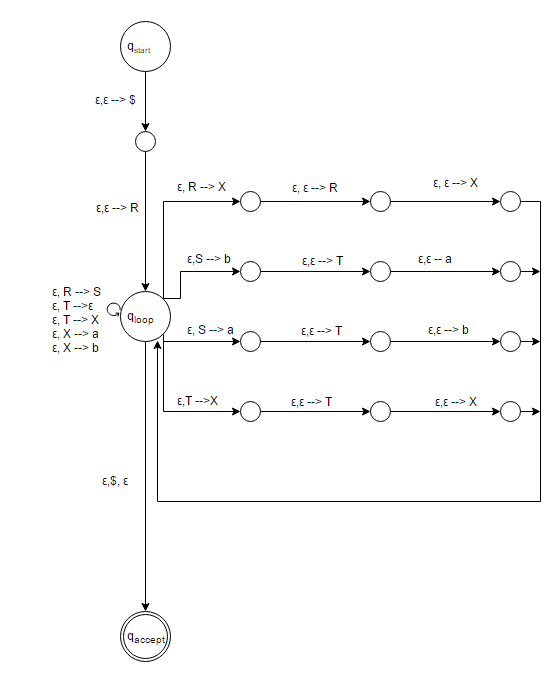
\includegraphics[scale = .75]{CFGtoPDA.png}
  		\label{fig:cfgtopda}
	\end{figure}

\section{Pumping Lemma with Regular Languages}
\subsection{}
	This langauge accepts some amount($\geq$ 0) of 0's followed by atleast 1, but no more than 2 \#, 			following by some amount ($\geq$ 0) of 0's or some amount of 0's followed by a \# then twice as 			many 0's as before\\
	$\lbrace$ 0$^{n}$ \# 0$^{2n}$ $\rbrace$

\subsection{}
	If G is a regular then there is a number P (Pumping length) such that S $\in$ and $\mid$S$					\mid$ $\geq$ P then S can be decomposed into S = XYZ S.T.: \\
		1.xy$^{i}$z $\in$ G\\
		2. $\mid$y$\mid$ $>$ 0 \\ 
		3. $\mid$xy$\mid$ $\leq$ P\\
		
	S = 0$^{p}$ \#  0$^{2p}$\\
	000\#000000\\
	y can only contain either the first set or the second set of 0's. If we pump up y we will have an    	incorrect amount of 0's on either side. Therefore G is not a regular language. 
	
\section{Chomsky Normal Form}
	A $\rightarrow$ BAB $\mid$ B $\mid$ $\epsilon$\\
	B $\rightarrow$ 00 $\mid$ $\epsilon$\\
	Add new start variable S$_{1}$ :\\
		S$_{0}$	$\rightarrow$ A\\
		A $\rightarrow$ BAB $\mid$ B $\mid$ $\epsilon$\\
		B $\rightarrow$ 00 $\mid$ $\epsilon$\\		
	Remove all $\epsilon$ :\\
		S$_{0}$	$\rightarrow$ A\\
		A $\rightarrow$ BAB $\mid$ BB $\mid$ AB $\mid$ BA $\mid$ A $\mid$ B \\
		B $\rightarrow$ 00\\
	Remove unit rules:\\
		S$_{0}$	$\rightarrow$ BAB $\mid$ BB $\mid$ AB $\mid$ BA $\mid$ 00\\
		A $\rightarrow$ BAB $\mid$ BB $\mid$ AB $\mid$ BA $\mid$ 00\\
		B $\rightarrow$ 00\\
	Add 'U' :\\
		S$_{0}$	$\rightarrow$ BAB $\mid$ BB $\mid$ AB $\mid$ BA $\mid$ 00\\
		A $\rightarrow$ BAB $\mid$ BB $\mid$ AB $\mid$ BA $\mid$ 00\\
		B $\rightarrow$ UU\\
		U $\rightarrow$ 0\\
	Simplify: \\
		S$_{0}$	$\rightarrow$ BA$_{1}$ $\mid$ BB $\mid$ AB $\mid$ BA $\mid$ 00\\
		A $\rightarrow$ BA$_{2}$ $\mid$ BB $\mid$ AB $\mid$ BA $\mid$ 00\\
		B $\rightarrow$ UU\\
		U $\rightarrow$ 0\\
		A$_{1}$ $\rightarrow$ SB\\
		A$_{2}$ $\rightarrow$ SB\\
		
\section{Pumping Lemma with Context-Free Languages}
\subsection{L = $\lbrace$ a$^{n}$ b$^{j}$ c$^{k}$ $\mid$ k = nj $\rbrace$}
	Assume L is a context free language. S = a$^{p}$ b$^{p}$ c$^{p^{2}}$\\
	S can be decomposed into S = uv$^{i}$xy$^{i}$z such that:\\
	1. uv$^{i}$xy$^{i}$z $\in$ L\\
	2. $\mid$ uy $\mid$ $\>$ 0 \\
	3. $\mid$ uxy $\mid$ $\leq$ P\\
	\\
	Cases:\\
	i. v contains b's or a's and y contains only c's. i = 0 so uv$^{0}$xy$^{0}$z 	thus making the string a$^{p}$ b$^{p}$ c$^{p^{2}-1}$ which is not in the language\\
	ii. v and y both contain a's and b's. i = 0 so uv$^{0}$xy$^{0}$z thus making the string a$^{p}$ b$^{p-k}$ c$^{p^{2}}$ or  a$^{p-k}$ b$^{p}$ c$^{p^{2}}$ which is not in the 		language\\ 
	iii. v and y both contain c's i = 0 making a$^{p}$ b$^{p}$ c$^{p^{2}-k}$ which is not in the language.\\
	iv. v and y contain 2 symbols. i = 2 uv$^{2}$xy$^{2}$z however the characters will be out of order and not in the language\\
	Thus L is not a CFG

\subsection{L = $\lbrace$ a$^{n}$ b$^{j}$ $\mid$ n $\geq$ (j - 1)$^{3}$ $\rbrace$}


	Assume L is a context free language. S = a$^{p}$ b$^{p}$\\
	S can be decomposed into S = uv$^{i}$xy$^{i}$z such that:\\
	1. uv$^{i}$xy$^{i}$z $\in$ L\\
	2. $\mid$ uy $\mid$ $\>$ 0 \\
	3. $\mid$ uxy $\mid$ $\leq$ P\\
	\\
	Cases:\\
	i. either v or y has more than one symbol. Thus when it is pumped up the characters are out of order and not in the language.\\
	ii. v contains only a's and y contains only b's. i = 2 thus making uv$^{2}$xy$^{2}$z which is not in the language, there are not enough a's
\end{document}